\IfFileExists{IEEEtran.cls}
  {\documentclass[conference]{IEEEtran}\newcommand{\realieee}{}}
  {\documentclass[10pt,a4paper,twocolumn]{article}}

\usepackage[T1]{fontenc}
\usepackage[utf8]{inputenc}
\usepackage{cite}
\usepackage{graphicx}
\usepackage{booktabs}
\usepackage[hidelinks]{hyperref}
\usepackage{url}


\ifdefined\realieee
  \IEEEoverridecommandlockouts
\else
  \usepackage{mathptmx}
  \usepackage[margin=0.72in,columnsep=0.25in]{geometry}
  \usepackage{caption}
  \captionsetup[table]{font=small,labelsep=newline,justification=centering,
                       singlelinecheck=false}
  \renewcommand{\thetable}{\Roman{table}}
  \renewcommand{\tablename}{TABLE}
  \newcommand{\IEEEauthorblockN}[1]{#1\\}
  \newcommand{\IEEEauthorblockA}[1]{\small #1}
  \date{}
  \newenvironment{IEEEkeywords}%
    {\vspace{4pt}\noindent\small\textbf{\textit{Keywords}}---\bfseries}{\par}
\fi


\renewcommand{\thesection}{\Roman{section}}
\renewcommand{\thesubsection}{\Alph{subsection}}
\makeatletter
\renewcommand{\@seccntformat}[1]{\csname the#1\endcsname.\hspace{0.5em}}
\renewcommand\section{\@startsection{section}{1}{\z@}%
  {1.8ex \@plus .8ex \@minus .2ex}%
  {0.8ex \@plus .2ex}%
  {\normalfont\normalsize\bfseries\scshape\centering}}
\renewcommand\subsection{\@startsection{subsection}{2}{\z@}%
  {1.5ex \@plus .6ex \@minus .2ex}%
  {0.5ex \@plus .2ex}%
  {\normalfont\normalsize\bfseries}}
\makeatother
\setlength{\textfloatsep}{8pt plus 2pt minus 2pt}


\begin{document}

\title{Modeling the Dynamics of Collective Intelligence Under Stress:\\
An AI-Based Framework for Predicting Adaptation\\
and Breakdown in Human--AI Groups}

\author{
\IEEEauthorblockN{Md Tazvir Rahat}
\IEEEauthorblockA{\textit{Dept. of Electrical and Computer Engineering}\\
\textit{North South University}\\
Dhaka, Bangladesh\\
tazvir.rahat@northsouth.edu}
\and
\IEEEauthorblockN{Mohammed Mushfiq Syed}
\IEEEauthorblockA{\textit{Dept. of Electrical and Computer Engineering}\\
\textit{North South University}\\
Dhaka, Bangladesh\\
mohammed.syed@northsouth.edu}
}

\maketitle

\begin{abstract}
Collective intelligence is usually measured as a single score, taken once,
under calm conditions. This study treats it instead as a trajectory and asks
whether the early interaction record of a group under stress indicates how
that group will end up. An agent-based model of a hidden-profile task was
built in which agents must pool distributed information items through
trust-weighted exchange, stress is a single load parameter that suppresses
both sending and accepting, and one human member is removed partway through
each run. Five conditions cross stress with the presence of a load-immune,
imperfectly reliable AI participant, with a size control. Each of 5{,}000
runs was labelled stable, adaptive, stressed or broken down from the
information state alone, and described by twelve features taken only from the
message log. A random forest reached a held-out macro-F1 of 0.34, against
0.21 for a model that knows only the condition, but within any single
condition the features did little better than chance. Every broken-down run
traced to a required item that only the removed member had held. In this
model, whether a group breaks down is settled mainly by which member it
loses, not by how it communicated beforehand.
\end{abstract}

\begin{IEEEkeywords}
collective intelligence, agent-based simulation, human--AI teams, stress,
early warning signals, hidden profile
\end{IEEEkeywords}

\section{Introduction}
 
Collective intelligence is the capacity of a group to solve problems more
effectively than its members acting alone, and the frameworks proposed for
studying it are numerous and only loosely connected \cite{suran2020}. It is a
group-level property rather than an aggregate of individual ability: meta-analytic evidence
indicates that the quality of a group's collaboration process predicts
collective performance roughly twice as strongly as the skill of its
individual members \cite{riedl2021}. How a group interacts matters more than
who is in it.
 
Almost all of this evidence, however, comes from quiet rooms. Participants
are strangers, sessions last about an hour, and nothing goes wrong. The
settings in which collective intelligence actually matters are the opposite:
epidemic response, flood evacuation, emergency resource allocation. In these
environments, groups face uncertainty, information overload, resource
scarcity and disrupted communication channels. Under such conditions a group
may reorganise and cope, or it may fragment. No current model predicts which.
 
The question has become more pressing because groups increasingly contain
artificial agents. That addition is not obviously beneficial. The largest
synthesis available reports that combining humans and AI often produces worse
decisions than the better party would have produced alone \cite{vaccaro2024}.
Whether this penalty grows or shrinks under stress is unknown, because the
underlying experiments were not conducted under stress.
 
\subsection{Research Objectives}
 
\textit{1) Simulate collective behaviour under stress:} construct an
agent-based model of a group solving a task that requires pooling distributed
information, across four conditions crossing stress with AI participation.
 
\textit{2) Define breakdown operationally:} produce a reproducible definition
of collective breakdown grounded in information integration and recovery,
independent of the interaction features used for prediction.
 
\textit{3) Identify structural indicators:} isolate features of the
interaction record that precede adaptation or breakdown.
 
\textit{4) Predict transitions:} train and evaluate models that classify
group state from early interaction structure, and report honestly whether
adaptation and breakdown are separable at all.
 
\subsection{Significance and Innovation}
 
The contribution is to treat collective intelligence as a trajectory rather
than a score, and to treat the definition of failure as a research problem
rather than an assumption. Existing measurement yields one number describing
how a group performed. This study models the group as an evolving interaction
structure and asks what state it will occupy next, so that intervention
becomes possible before failure rather than diagnosis after it.

\subsection{Summary of Findings}

The model was built, calibrated on reserved seeds, and used to generate
5{,}000 labelled runs. Stress had a clear effect on outcomes: it almost
eliminated early completion and pushed a quarter to a third of runs into
prolonged partial integration. Classifiers trained on the early message log
beat every naive baseline, but most of what they learned was which
condition a run belonged to. Within a condition, and between adaptation and
breakdown in particular, they did little better than chance. The reason is
structural and is traced in Section~V: breakdown in this model is decided at
the moment of the perturbation by whether the lost member held something no
one else did. Section~II reviews the literature, Section~III describes the
methodology as implemented, Section~IV reports results, and Sections~V and~VI
discuss them and set out what should change next.
 
\section{Literature Review}
 
Research bearing on this study is distributed across communities that
rarely cite one another: the psychometric measurement of collective
intelligence, organisational research on teams under stress, human--AI
interaction, network science, and the complex-systems literature on critical
transitions. This review synthesises them thematically and locates the gap at
their intersection.
 
\subsection{Scope and Search Strategy}
 
Searches were conducted in August 2026 across Google Scholar, arXiv, Semantic
Scholar and PubMed, with direct retrieval from \emph{Nature}, \emph{Science},
Springer and IEEE Xplore. Representative Boolean strings were
\texttt{"collective intelligence" AND (stress OR crisis OR breakdown)},
\texttt{("human-AI" OR "human-agent") AND (team OR collective) AND
performance}, \texttt{("threat rigidity" OR "team resilience") AND
coordination}, and \texttt{("agent-based" OR simulation) AND (validation OR
"early warning")}. Backward and forward citation chaining was applied to the
foundational works \cite{woolley2010, riedl2021}.
 
Peer-reviewed empirical studies, meta-analyses, systematic reviews and
methodological papers were included, together with recent preprints where no
peer-reviewed equivalent exists. Studies of individual performance without a
group comparison, commercial sources and non-peer-reviewed commentary were
excluded. Screening proceeded from title to abstract to full text.
 
\subsection{Collective Intelligence as a Static Measurement}
 
Woolley et al.\ \cite{woolley2010} administered batteries of tasks to 699
participants working in groups of two to five and identified a single factor,
$c$, explaining much of the variance in performance across otherwise
unrelated tasks. The correlates proved more surprising than the factor
itself. Average member intelligence predicted $c$ only weakly, while the
average social sensitivity of members, the evenness of speaking-turn
distribution and the proportion of women in the group predicted it
considerably better.
 
Riedl et al.\ \cite{riedl2021} revisited the question meta-analytically
across 22 studies comprising 1{,}356 groups and 5{,}279 participants.
Evidence for a general collective intelligence factor survived leave-one-out
testing, and collaboration-process measures carried approximately twice the
predictive weight of individual member skill.
 
The finding is contested rather than settled. Bates and Gupta
\cite{bates2017} reported across three studies with 312 participants that
individual IQ accounted for approximately 80 per cent of the variance in
group-level performance, with no detectable relationship to gender balance or
turn-taking. This study takes no position on that dispute, since its
subject is how collective performance \emph{changes} under load rather than
whether a general factor exists.
 
What both camps share is more consequential here. Collective
intelligence is treated throughout as a quantity a group possesses: a score
obtained from a single session, under conditions deliberately kept calm,
among strangers with no prior history. A score describes an endpoint. It
cannot describe a trajectory, and it cannot indicate when a group began to
fail.
 
\subsection{Stress and the Loss of Shared Knowledge}
 
Ellis \cite{ellis2006} supplies the mechanism on which this study rests.
Across 97 teams performing a command-and-control simulation, acute stress
degraded shared mental models and transactive memory---the distributed
awareness of who knows what---and that degradation statistically explained
the resulting performance loss. The failure was structural rather than
motivational: members continued working, but the group's shared
representation of its own knowledge came apart. This identifies what to
measure. If stress destroys the routing of knowledge rather than the effort
of individuals, breakdown should be observable as a failure of information to
reach the members who need it.
 
The wider stress literature is considerably less consistent. Threat-rigidity
theory \cite{staw1981} predicts two specific responses to perceived threat: a
restriction in information processing and a constriction of control as
authority centralises upward. Yet Driskell and Salas \cite{driskell1991}
tested centralisation against an increased-receptivity hypothesis and found
the latter, with participants of both high and low status becoming more
willing to defer to a partner's judgement under stress.
 
Mojzisch et al.\ \cite{mojzisch2025}, reviewing fifty years of experimental
work on group decision making under acute stress, attribute much of this
inconsistency to methodology. Studies rarely employ validated stress
inductions, routinely conflate stress with time pressure, and frequently
measure individual choices made inside a group rather than genuine collective
decisions. They report no empirical support for groupthink's central claim
regarding cohesion, and describe group-level evidence for threat-rigidity as
mixed at best. Their recommendations shape this study in two ways. Stress
is operationalised as a single controlled parameter rather than conflated
with time pressure, mirroring the separation that validated human instruments
such as the group version of the Trier Social Stress Test
\cite{vondawans2011} achieve in laboratory settings. The task possesses an
objectively correct answer, following the hidden-profile paradigm of Stasser
and Titus \cite{stasser1985}. In a hidden profile, the information required
to identify the correct option is distributed such that no member can reach
it alone, making information sharing both necessary for success and directly
measurable.
 
A separate literature offers a vocabulary for the group's response to that
load rather than for the load itself. Stoverink et al.\ \cite{stoverink2020}
draw on conservation-of-resources theory to model team resilience as a
capacity that resides in the team as a whole: built up jointly from
resources members hold in common, and unfolding through the team's ongoing
processes rather than fixed in advance. Their starting observation is that
teams under sustained adversity either recover their functioning or instead
see their coordination break down and their output decline, and the model is
an attempt to explain what separates the two. That same pairing, adaptation
against breakdown, is what the present study makes measurable through the
interaction record rather than through resource-based indicators, treating
it as a trajectory a group is on rather than a trait it either has or lacks.
 
\subsection{Human--AI Collectives Under Load}
 
Peeters et al.\ \cite{peeters2021} argue that in mixed human--AI systems the
significant risks emerge at the collective level rather than in any single
component, which is also the premise of this study. The empirical record
counsels caution. Vaccaro et al.\ \cite{vaccaro2024}
conducted a preregistered systematic review and meta-analysis of 106
experimental studies reporting 370 effect sizes, finding that human--AI
combinations performed on average worse than whichever of the two performed
better alone. Losses concentrated in decision-making tasks while gains
appeared in content creation, and design features in which the field has
invested heavily---displaying explanations, showing model confidence---did
not moderate the outcome. Two properties of that corpus define the gap this
study enters: it is overwhelmingly dyadic, pairing a single person with a
single model, and it contains almost no sustained stress.
 
Burton et al.\ \cite{burton2024} identify a failure mode specific to the
collective level. When many members of a group consult the same small number
of language models, privately held beliefs converge and the diversity on
which collective intelligence depends erodes before deliberation begins.
Premature consensus is particularly dangerous because, observed from outside,
it is difficult to distinguish from efficient coordination.
 
Shiiku et al.\ \cite{shiiku2025} demonstrate that these effects are
time-dependent. Running an iterative storytelling task across $5\times5$ grid
networks under human-only, AI-only and mixed configurations, they found that
AI-only networks initially produced work rated more creative and more
diverse, but that mixed networks overtook them on diversity across successive
iterations. A single measurement taken at either end of that experiment would
have supported the opposite conclusion, which constitutes a direct argument
for temporal modelling.
 
Taken together, these findings suggest a mechanism worth testing rather than
assuming. An artificial participant does not experience stress and does not
reduce its output as load rises. Its contributions therefore occupy a growing
share of group communication precisely when human members are least able to
scrutinise them. If that agent is imperfectly reliable, stress should amplify
the propagation of its errors.
 
\subsection{Network Structure and Position}
 
Structure carries substantial explanatory weight independent of composition.
Shirado and Christakis \cite{shirado2017} showed that autonomous agents
behaving with a small degree of randomness improved a human group's ability
to solve a distributed coordination problem, but that the magnitude of the
benefit depended on where in the network those agents were placed. Centola
\cite{centola2022} synthesises the wisdom-of-crowds and
collective-problem-solving traditions and concludes that on difficult tasks,
decentralised and informationally inefficient networks tend to outperform
densely connected ones, because slower information flow protects unusual
ideas long enough for them to be evaluated rather than suppressed. Cui and
Yasseri \cite{cui2024} formalise such collectives as multilayer networks
with distinct cognition, physical and information layers, the closest
existing formalism to the representation required here. The size of the
units in which people interact also matters: Iacopini et al.\
\cite{iacopini2022} show that interactions in groups, rather than in pairs,
change how large a committed minority must be before a population tips to a
new convention.
 
These questions are operational rather than abstract in the settings that
motivate this work, where AI already supports disease surveillance and
emergency logistics \cite{haykal2025} and climate action increasingly
depends on coordinating distributed citizen, non-governmental and
government actors \cite{gonzalo2023}.
 
\subsection{Detecting Transitions Before They Complete}
 
Two technical literatures supply the modelling apparatus. Temporal graph
learning has matured rapidly, with memory-based architectures such as
Temporal Graph Networks \cite{rossi2020} maintaining per-node state updated
by each interaction. These models are well benchmarked, but almost entirely
on dynamic link prediction and anomaly detection. Classifying the state of an
entire graph as it evolves---which is what the question ``is this group
stable, adapting, or breaking down?'' amounts to---remains comparatively
undeveloped.
 
Early-warning-signal theory supplies the other half. George et al.\
\cite{george2023} review critical slowing down: as a system approaches a
bifurcation it recovers more slowly from perturbation, and this appears in
observable time series as rising variance and rising lag-1 autocorrelation.
The phenomenon has been demonstrated across ecosystems, financial markets,
climate records and the onset of epileptic seizures. Rietkerk et al.\
\cite{rietkerk2025} add a qualification that any applied system must handle:
the same signals also precede transitions that are not catastrophic, so their
presence indicates an approaching change of regime rather than an approaching
failure. Distinguishing the two is part of the problem rather than a detail.
 
The relevance here is methodological as well as theoretical. If recovery time
distinguishes systems near collapse from systems merely disturbed, then
adaptation and breakdown---which resemble one another closely at the moment
of disruption, since both involve structural reorganisation---may be
separable by what follows the disruption rather than by the disruption
itself. This motivates introducing a controlled perturbation mid-run and
measuring whether information flow resumes.
 
\subsection{Validity Constraints on Simulated Data}
 
Because the data for this study are generated by simulation, one
methodological constraint is binding. Larooij and T\"ornberg
\cite{larooij2025} reviewed generative agent-based models and concluded that
validation, not expressiveness, is the field's central problem. They document
black-box model structure, cultural bias inherited from training data,
unpredictable behaviour on out-of-distribution scenarios, and validation
procedures in which a model effectively adjudicates the plausibility of its
own output. Their argument is not that such simulations are useless, but that
a simulated dataset carries no evidential weight unless its validation
strategy is fixed in advance.
 
This study accepts that standard. Labelling criteria and thresholds were
fixed on a reserved set of calibration seeds before the study dataset was
generated, and were not revised after any classifier was trained;
sensitivity across threshold values is reported; and the agent rules are
deliberately simple and inspectable rather than language-model-based, so that
any observed transition can be traced to the rule that produced it.
 
\begin{table}[t]
\caption{Research Gaps and Corresponding Design Decisions}
\label{tab:gaps}
\centering
\footnotesize
\setlength{\abovecaptionskip}{3pt}
\setlength{\belowcaptionskip}{3pt}
\renewcommand{\arraystretch}{0.95}
\begin{tabular}{@{}p{3.3cm}p{4.3cm}@{}}
\toprule
\textbf{Gap identified} & \textbf{How this study responds} \\
\midrule
Measured as a static score under calm conditions \cite{woolley2010,riedl2021}
& Interaction structure observed across time under rising stress \\
Stress damage inferred from outcomes, not observed \cite{ellis2006}
& Integration measured directly: which required items reach a decision-maker \\
Human--AI evidence dyadic, unstressed \cite{vaccaro2024,burton2024}
& Multi-agent groups with a load-immune, imperfectly reliable AI participant \\
Structure known to matter but not tracked under load \cite{shirado2017,centola2022}
& Full message log retained; structure computed from it over any window \\
No operational definition of breakdown, hence no training labels
& Breakdown defined from integration after a controlled perturbation \\
Simulated data lacks validation \cite{larooij2025}
& Thresholds fixed on reserved seeds; labels and features kept strictly separate \\
\bottomrule
\end{tabular}
\end{table}
 
\subsection{Research Gaps and Unique Contributions}
 
Table~\ref{tab:gaps} maps the gaps identified above onto the design decisions
that follow from them. Four contributions result.
 
\textit{1) Structural observation under load:} the group is represented as a
temporal interaction structure and observed while stress is applied, so that
degradation is measured in the coordination itself rather than inferred from
a final score.
 
\textit{2) An operational definition of breakdown:} a group is classified as
broken down when the information required for the correct answer can no
longer be assembled by any member following a controlled perturbation.
Stable, adaptive and stressed states are defined by the same measure at
differing levels of severity and recovery. Because the standard
literature offers no such definition, producing a defensible one is treated
as a contribution in its own right rather than a preliminary step.
 
\textit{3) Separation of labels from features:} outcome labels derive
exclusively from which required information items arrived and when;
predictive features derive exclusively from the message log. This separation
prevents the circularity that would otherwise inflate accuracy without
establishing anything.
 
\textit{4) An honest test of separability:} the study reports whether
adaptation and breakdown can in fact be distinguished from early interaction
structure. A negative result---that the two are not separable at the horizons
examined---was planned for as a legitimate outcome, and it is the result
obtained.
 
\section{Methodology}
 
This study is conducted entirely in simulation. No human participants are
involved, so no ethical approval is required. The trade-off is accepted
deliberately: agent-based simulation permits the thousands of controlled
runs that supervised learning requires, at the cost of psychological
realism. Section~V-C states the resulting limits.

The methodology below is the one implemented. Where it departs from the
original proposal, the departure and its reason are stated at the point
where it occurs. Parameter values are collected in Table~\ref{tab:params}.
 
\subsection{Research Design}
 
The experiment crosses two factors, giving four primary conditions: group
composition (human-only, human plus AI) by stress level (calm, stressed).
Stress is applied identically across composition conditions, so AI presence
is the only variable distinguishing them.
 
A fifth control condition contains one additional human agent in place of the
AI agent. Without it, any difference between composition conditions could be
attributed to group size rather than to the presence of an artificial
participant. C4 and C5 therefore have the same number of agents and the same
number of items, and differ only in what the thirteenth participant is.
Table~\ref{tab:design} summarises the design. The design has no size control
under calm conditions; a supplementary check that supplies one is reported in
Section~IV-B.
 
\begin{table}[t]
\caption{Experimental Conditions}
\label{tab:design}
\centering
\footnotesize
\setlength{\abovecaptionskip}{3pt}
\setlength{\belowcaptionskip}{3pt}
\renewcommand{\arraystretch}{0.95}
\begin{tabular}{@{}llll@{}}
\toprule
\textbf{Condition} & \textbf{Humans} & \textbf{AI} & \textbf{Stress} \\
\midrule
C1 Human-only, calm      & 12 & 0 & 0.10 throughout \\
C2 Human-only, stressed  & 12 & 0 & 0.10 $\rightarrow$ 0.32 \\
C3 Human+AI, calm        & 12 & 1 & 0.10 throughout \\
C4 Human+AI, stressed    & 12 & 1 & 0.10 $\rightarrow$ 0.32 \\
C5 Size control, stressed & 13 & 0 & 0.10 $\rightarrow$ 0.32 \\
\bottomrule
\end{tabular}
\end{table}
 
\subsection{Task Environment}
 
Each run instantiates a hidden-profile task \cite{stasser1985}. Every agent,
the AI included, starts with three information items, so a group of twelve
humans holds 36 and a group of thirteen agents holds 39. Twelve of those
items are drawn at random as the required set. The correct option becomes
identifiable when all twelve reach a single agent. No agent starts with more
than three, so no agent can reach the answer alone. Items are integer
identifiers; the simulation carries no natural-language content, and the
semantic framing exists only in the write-up.

The proposal specified that each item be held by more than one agent from
the start, so that removing an agent could never destroy information. The
implementation does the opposite: every item has exactly one holder at
initialisation, and copies exist only once agents have passed them on. The
reason is that redundancy handed out in advance would make a group's
resilience to losing a member a property of the set-up rather than of the
group. With a single initial holder, how much a group stands to lose at the
perturbation depends on how much it has already shared, which is the group's
own doing. The cost of this choice is that a perturbation can destroy a
required item outright, and Section~IV shows how much that cost matters.
 
\subsection{Agent Model}
 
A human agent is defined by three state variables: the set of items it holds,
a vector of trust values toward every other agent, and a scalar load in
$[0,1]$ representing cognitive burden.
 
Each run lasts 1{,}000 ticks. At every tick the living agents act once each,
in random order. An agent $s$ with load $L_s$ transmits with probability
\begin{equation}
p_{\mathrm{send}} = r\,(1 - L_s), \qquad r = 0.30,
\end{equation}
choosing one of its items uniformly at random. The recipient is drawn from
all other agents with probability proportional to $s$'s trust in each,
$T_{s j}$. The recipient $j$ accepts with probability
\begin{equation}
p_{\mathrm{accept}} = T_{j s}\,(1 - L_j)\,w_s ,
\end{equation}
where $w_s$ is the AI trust weight if $s$ is the AI and 1 otherwise. An
accepted item is added to the recipient's holdings; agents have no capacity
limit. After each attempt, the sender adjusts its trust in that recipient:
up by 0.05 after an acceptance, capped at 1, and down by 0.02 after a
refusal, floored at 0.05. Trust starts at 0.50 in every direction. An
agent's trust in a partner therefore changes only through its own attempts
to send to that partner.

The asymmetry between the increment and the decrement was introduced during
calibration. With symmetric steps, trust rises only if more than half of
attempts succeed. Under load that rate was out of reach, trust drained to
the floor in every condition, and no group functioned. The floor is above
zero so that a route that has gone quiet can still be tried again.
 
Recovery after perturbation is not implemented as a rule. No instruction
directs an agent to compensate for a lost member. Recovery, where it occurs,
emerges from trust updating and trust-weighted partner selection: failed
transmissions to an absent agent lower its trust score, and remaining agents
consequently redistribute traffic toward reachable partners. Whether this
suffices to restore information flow depends on prevailing load, which is
precisely the effect under study.
 
The AI agent differs in exactly three respects, and these constitute the
operational definition of an artificial participant in this model:
 
\textit{1) Load immunity:} its load stays at the calm value of 0.10 whatever
the stress schedule, reflecting that computational systems do not experience
social or cognitive stress \cite{peeters2021}.
 
\textit{2) Imperfect reliability:} on 15 per cent of its transmissions the
AI sends a well-formed item identifier that it does not hold, drawn from a
reserved range that can never collide with a genuine item. Recipients cannot
tell the difference, and such items never count towards integration. This
operationalises the mechanism suggested by the meta-analytic finding that
human--AI combinations frequently underperform the stronger party alone
\cite{vaccaro2024}.
 
\textit{3) Distinct trust weighting:} acceptance of AI-originated items is
multiplied by a separate weight $w$, permitting over- and under-reliance to
be modelled independently of inter-human trust \cite{burton2024}. In this
study $w = 1$, the neutral value; sweeping it is left to future work.

Because agents have no capacity limit and items carry no content, a false
item costs the group only the transmission it occupied. It cannot displace a
genuine item or mislead a recipient. The AI's unreliability is therefore a
weak manipulation in this implementation, and Section~V returns to what that
means for the AI results.
 
\subsection{Stress Schedule}
 
Stress is operationalised as the load parameter of human agents. Calm
conditions hold load at 0.10 for the full run. Stressed conditions start at
the same 0.10, rise linearly between ticks 10 and 50 to 0.32, and hold that
value to the end. The schedule is identical in C2, C4 and C5.

Because load reduces both sending and accepting, its effect on a single
exchange compounds: at peak load a human-to-human exchange succeeds at
$(0.68/0.90)^2 \approx 0.57$ of its calm rate, before any change in trust.
The proposal did not fix a peak value. An earlier setting of 0.45 was
rejected during calibration because it stalled stressed groups short of the
required set so reliably that the adaptive state was left almost empty.
 
This is a deliberate simplification and is claimed as such. Load is not a
model of human stress physiology; it is a single controlled parameter that
degrades transmission and reception, following the recommendation that stress
manipulations be separated from time pressure rather than conflated with it
\cite{mojzisch2025}.
 
\subsection{Perturbation}
 
At tick 55 in every run, five ticks after the stress ramp completes, one
human agent is chosen uniformly at random and removed. Items held only by
that agent become unreachable; items it had already passed on remain in
circulation. Remaining agents receive no notification and continue operating
under unchanged rules. They keep choosing the absent agent as a recipient,
every such attempt fails, and trust in that route falls until traffic moves
elsewhere.
 
The perturbation is held constant across all conditions so that differences
in recovery are attributable to condition rather than to disturbance type.
Its purpose follows from early-warning-signal theory: systems approaching a
critical transition recover more slowly from disturbance than systems that
are merely perturbed \cite{george2023}. Since adaptation and breakdown
resemble one another at the moment of disruption, the discriminating
information lies in what follows.
 
In human+AI conditions the removed agent is always human, so that AI presence
is held constant across the perturbation.

One consequence of the random choice needs stating plainly, because it turns
out to dominate the results. If the removed agent was, at tick 55, the only
holder of any required item, the correct option can never be assembled in
that run.
 
\subsection{Outcome Labelling}
 
Labels are derived exclusively from the information state and never from the
communication record. This separation is the central methodological
commitment of the study: since the predictive features are drawn from the
communication record, defining outcomes in those same terms would make the
prediction task circular and inflate accuracy without establishing anything.
 
\emph{Integration} $I(t)$ is the number of required items held by the
best-informed living agent at tick $t$, out of $N = 12$. The AI's holdings
count, since it is a member of the group; false items never count. Let
$t^{*}$ be the first tick at which $I(t) = N$, if there is one. Four states
are assigned, checked in this order:

\begin{itemize}\itemsep2pt
\item \textbf{Broken down:} a required item was destroyed at the
      perturbation, or the run ends with $I(T) < 0.6N$. The correct option is
      never identifiable.
\item \textbf{Stressed:} nothing was destroyed and $I(T) \ge 0.6N$, but
      $I(t)$ never reaches $N$. Partial arrival continues without completion.
\item \textbf{Stable:} $t^{*} \le 450$. The group completes the task early,
      and the perturbation does not visibly delay it.
\item \textbf{Adaptive:} $t^{*} > 450$. The group completes the task, but
      only late, after absorbing the loss.
\end{itemize}

This is a departure from the proposal, which defined recovery as the rate of
required-item arrival returning to a fraction of its pre-perturbation level.
Calibration showed that measure to be unusable. Arrival slows as the best
desk fills, whatever else happens, because fewer required items remain to
arrive. The smoothed arrival rate peaked during the first 30 ticks and then
fell steadily in calm and stressed runs alike, so it never ``returned'' in
either and could not separate them. Time to completion captures the same
idea---how long a group takes to recover full integration after losing a
member---without depending on the shape of a saturating curve.

Following the requirement that simulated datasets carry no evidential weight
absent a pre-specified validation strategy \cite{larooij2025}, both
thresholds (tick 450 and the 60 per cent floor) were fixed on calibration
seeds and were not revised after any model was trained. Completion times
form a single broad hump, rising from tick 182 to a peak near tick 575 and
then tailing off flat to the end of the run, with no gap anywhere that would
justify placing the stable threshold in it. Sensitivity across a grid of
both thresholds is reported instead.

\subsection{Calibration}

Seeds 0 to 299 were reserved for calibration and never enter the study
dataset. Five checks were run on them before any study data were kept:
whether stress produced a visible gap in integration between C1 and C2;
whether all four states were populated; whether the AI was so often the
best-informed agent that ``the group integrated the information'' would
really mean ``the AI did''; whether the calm AI effect survived an added
calm size control; and how much redundancy groups had built by the
perturbation tick.

Three provisional values were changed as a result. The required set was
reduced from 16 items to 12, the run was lengthened from 800 ticks to
1{,}000, and the peak load was lowered from 0.45 to 0.32. At the provisional
values stressed groups almost never completed, which left the adaptive and
stable states nearly empty under stress. The revised values were chosen by
sweeping the required set (12--16), the run length (800--1{,}400) and the
peak load (0.26--0.45) on calibration seeds and taking the combination under
which every state appeared somewhere in the design while the stress effect
remained clear. A first study dataset had been generated at the provisional
values; it was discarded when the values changed. No classifier had been
trained on it.
 
\subsection{Feature Extraction}
 
Features are computed exclusively from the message log over an initial
window of each run, so that prediction precedes the outcome being predicted.
The primary window is ticks 0--199, the first fifth of the run. It contains
the perturbation at tick 55 and the first 145 ticks of the group's response.
A window ending at the perturbation would contradict the argument of
Section~II-F, that adaptation and breakdown differ in what follows the
disruption rather than in the disruption itself. A window much longer would
start to overlap the outcome: in the study data only 5 of 5{,}000 runs
completed the task inside the first 200 ticks. The window length was chosen
on calibration seeds, and the prediction-horizon analysis in Section~III-J
reports every shorter window as well.

Five families are extracted:
 
\textit{1) Volume:} total transmissions, mean transmissions per tick, and the
slope of the transmission rate.
 
\textit{2) Distribution:} Gini coefficient of transmissions per agent, count
of silent agents, and the ratio of most to least active agent.
 
\textit{3) Structure:} number of connected components in the interaction
graph, graph density, and degree centralisation \cite{shirado2017,
centola2022}.
 
\textit{4) Reciprocity:} proportion of transmissions followed by a
transmission in the reverse direction, and mean delay to reciprocation.
 
\textit{5) Instability:} rolling variance of transmission rate and lag-1
autocorrelation of transmission rate, these being the observable signatures
of critical slowing down \cite{george2023}.
 
In human+AI conditions, two further features record the proportion of
AI-originated items accepted and the ratio of AI-to-human against
human-to-human traffic. Both are zero in human-only runs.

No feature references item identity, integration, or task outcome. This is
enforced rather than merely checked: before extraction, each logged message
is reduced to five fields---tick, sender, recipient, whether it was
accepted, and whether the sender was the AI---so the extraction code never
receives the item identifier or the flag marking a false item.

Three of the fifteen features were dropped before modelling. The count of
silent agents was 0 and the number of connected components was 1 in every
run: at these parameters every agent speaks and the interaction graph is
always connected within the window. Mean transmissions per tick is the total
divided by a fixed window length, so it duplicates the total exactly. Twelve
features remain.
 
\subsection{Predictive Modelling}
 
Each run yields one fixed-length feature vector and one label, so the
prediction task is multi-class classification over tabular data rather than
sequence or graph learning. Although temporal graph architectures exist for
evolving networks \cite{rossi2020}, they address dynamic link prediction
rather than whole-graph state classification, and applying them to a
fixed-length summary per run would add complexity without a corresponding
gain in what can be concluded.
 
Two classifiers are therefore trained: multinomial logistic regression on
standardised features, selected for interpretability of coefficients, and a
random forest of 300 trees with at least five runs per leaf, selected for
its tolerance of non-linear feature interactions. Both weight classes
inversely to their frequency, since the stable state is rare. Feature
importance is measured by permutation on the held-out set, as the drop in
macro-F1 when one feature is shuffled; this serves objective three directly.

Two baselines were planned. A majority-class predictor establishes the
floor. A single-feature logistic regression on transmission volume alone
establishes whether the structural and instability features contribute
anything beyond a naive measure of activity. If the full models do not
exceed this second baseline, that result is reported as the finding.

Two comparisons were added once the design was implemented. A
\emph{condition-only} model is a logistic regression on the five condition
indicators and nothing else. Stress changes message volume substantially,
so a feature model can score well merely by recognising whether a run was
stressed; the condition-only model measures how far that alone goes. An
\emph{information-state ceiling} fits the same random forest to four
quantities the predictors are forbidden to see, all known by the end of the
feature window: integration at tick 199, the number of items still held by
a single agent at the perturbation, how many of the removed agent's original
items had not been shared, and whether a required item was destroyed. No
model of the message log can be expected to beat this ceiling, so it
indicates how much of the outcome is settled by tick 200 at all.
 
\subsection{Evaluation}
 
The 5{,}000 runs are split 80/20 into training and held-out test sets,
stratified by label, with a fixed split seed. Five-fold stratified
cross-validation is run on the training partition, and the held-out set is
touched once per model. Reported metrics are accuracy, macro-averaged F1,
per-class precision and recall, and the full confusion matrix.
Macro-averaging is specified because class frequencies differ across
conditions and overall accuracy would otherwise be dominated by the majority
state.

Four analyses go beyond headline accuracy. The first three were planned; the
fourth was added for the same reason as the condition-only baseline.
 
\textit{1) Adaptive versus broken-down separability.} These two states are
the difficult pair, since both involve structural reorganisation following
disturbance. Binary classification restricted to these classes is reported
separately, as aggregate accuracy would otherwise conceal failure on the case
of interest.
 
\textit{2) Prediction horizon.} Models are retrained on features computed
over windows ending at ticks 55, 100, 150 and 200, to establish how early a
state becomes predictable and whether seeing the response to the
perturbation adds anything. The window ending at tick 55 contains no
post-perturbation data at all.
 
\textit{3) Threshold sensitivity.} Labels are recomputed for every
combination of stable threshold (ticks 350, 450, 550) and breakdown floor
(60, 70, 80 per cent) and the models retrained. A conclusion that holds only
at one threshold value is reported as an artefact rather than a finding.

\textit{4) Within-condition prediction.} Models are cross-validated inside
each condition separately, where recognising the condition cannot help, and
compared with a classifier that guesses in proportion to class frequency.
 
\begin{table}[t]
\caption{Simulation and Evaluation Parameters}
\label{tab:params}
\centering
\footnotesize
\setlength{\abovecaptionskip}{3pt}
\setlength{\belowcaptionskip}{3pt}
\renewcommand{\arraystretch}{0.95}
\begin{tabular}{@{}p{3.1cm}p{2.3cm}p{2.0cm}@{}}
\toprule
\textbf{Parameter} & \textbf{Value} & \textbf{Range tested} \\
\midrule
Human agents per group, $n$  & 12 & 12--13 \\
Items per agent (total)      & 3 (36 or 39) & --- \\
Required items, $N$          & 12 & 12--16$^{a}$ \\
Holders per item at start    & 1 & --- \\
Ticks per run                & 1{,}000 & 800--1{,}400$^{a}$ \\
Runs per condition           & 1{,}000 & --- \\
Base transmission rate $r$   & 0.30 & --- \\
Load, calm                   & 0.10 & --- \\
Load, stressed start / peak  & 0.10 / 0.32 & peak 0.26--0.45$^{a}$ \\
Stress ramp                  & ticks 10--50 & --- \\
AI false-item rate           & 0.15 & 0--0.15$^{b}$ \\
AI trust weight $w$          & 1.0 & --- \\
Initial trust                & 0.50 & --- \\
Trust up / down / floor      & 0.05 / 0.02 / 0.05 & --- \\
Perturbation tick            & 55 & --- \\
Feature window               & ticks 0--199 & 55--200 \\
Stable threshold on $t^{*}$  & 450 & 350--550 \\
Breakdown floor, $I(T)/N$    & 0.60 & 0.60--0.80 \\
Train / test split           & 80 / 20 & --- \\
Cross-validation folds       & 5 & --- \\
Calibration seeds            & 0--299 & --- \\
Study seeds                  & 10{,}000--14{,}999 & --- \\
\bottomrule
\multicolumn{3}{@{}p{7.4cm}@{}}{\scriptsize $^{a}$On calibration seeds only.
$^{b}$Supplementary check, Section~IV-B.}
\end{tabular}
\end{table}
 
\subsection{Implementation}
 
The simulation is implemented in Python with deterministic seeding, so that
any run can be reproduced exactly and any observed transition traced to the
rule that produced it. Classifiers use scikit-learn. One script generates
the dataset and writes the predictors, the labels and the information-state
quantities to separate files; a second trains and evaluates every model
reported below. Re-running both regenerates every number in Section~IV.

\section{Results}

\subsection{The Dataset}

Table~\ref{tab:labels} gives the share of runs in each state. Stress had the
effect the study depends on. Under calm conditions a quarter of human-only
groups completed early and almost none stalled; under stress early
completion all but disappeared, falling to about one per cent, and a quarter
to a third of runs ended stalled short of the full set. Stress also raised
the rate of breakdown in human-only groups from 25.3 to 30.7 per cent.

\begin{table}[t]
\caption{Share of Runs in Each State (1{,}000 Runs per Condition)}
\label{tab:labels}
\centering
\footnotesize
\setlength{\abovecaptionskip}{3pt}
\setlength{\belowcaptionskip}{3pt}
\renewcommand{\arraystretch}{0.95}
\begin{tabular}{@{}lcccc@{}}
\toprule
\textbf{Condition} & \textbf{Stable} & \textbf{Adaptive} & \textbf{Stressed} & \textbf{Broken} \\
\midrule
C1 Human-only, calm      & 0.259 & 0.488 & 0.000 & 0.253 \\
C2 Human-only, stressed  & 0.011 & 0.425 & 0.257 & 0.307 \\
C3 Human+AI, calm        & 0.165 & 0.599 & 0.010 & 0.226 \\
C4 Human+AI, stressed    & 0.008 & 0.382 & 0.355 & 0.255 \\
C5 Size control, stressed & 0.008 & 0.402 & 0.319 & 0.271 \\
\midrule
All runs                 & 0.090 & 0.459 & 0.188 & 0.262 \\
\bottomrule
\end{tabular}
\end{table}

Every one of the 1{,}312 broken-down runs was broken down for the same
reason: the removed agent had been the only holder of at least one required
item. The 60 per cent floor on final integration never decided a label.
This is the single most important fact about the dataset. It means the
broken-down state records a loss at tick 55, not a failure to integrate
afterwards. Stress raises the rate of such losses indirectly. By the
perturbation tick, calm human-only groups had left 9.9 items on average with
a single holder, and stressed ones 11.8, because the stress ramp had already
cut how much they passed on.

\subsection{Effect of the AI Participant}

Under stress the AI made little difference. C4 and C5 differ by at most 3.6
percentage points in any state, and each share has a standard error of
about 1.5 points at 1{,}000 runs, so none of those differences is clearly
outside chance. The largest is a higher share of stalled runs with the AI
(35.5 against 31.9 per cent).

Under calm conditions C3 completed early less often than C1 (16.5 against
25.9 per cent). Because the design has no calm size control, a
supplementary check ran 1{,}000 further runs of each of four calm
configurations on seeds 20{,}000--20{,}999, outside both the calibration and
study ranges. Early completion was 26.6 per cent with twelve humans, 19.2
per cent with thirteen, 18.6 per cent with twelve humans and an error-free
AI, and 16.1 per cent with the standard AI. Most of the drop is therefore an
effect of group size. A thirteenth participant, human or not, adds three
items to the pool and one more partner for every sender to divide its
attention between, which probably explains the slower completion. The AI's
errors account for a further two to three points, which is at the edge of
what 1{,}000 runs can resolve.

One difference does favour the AI conditions, and it is mechanical. The AI
is never removed, so required items it holds can never be destroyed. Human+AI
groups broke down less often than human-only groups at the same stress
level (22.6 against 25.3 per cent calm, 25.5 against 30.7 per cent stressed).

\subsection{Four-Class Prediction}

Table~\ref{tab:models} reports the main comparison. Both feature models beat
the majority-class floor and the volume-only baseline, which was the
planned test of whether structure adds anything to activity. The random
forest reached a held-out macro-F1 of 0.341 against 0.249 for volume alone.

\begin{table}[t]
\caption{Four-Class Results. CV: Mean $\pm$ SD Macro-F1 Over Five Folds of
the Training Set. Test: Held-Out 20 Per Cent}
\label{tab:models}
\centering
\footnotesize
\setlength{\abovecaptionskip}{3pt}
\setlength{\belowcaptionskip}{3pt}
\renewcommand{\arraystretch}{0.95}
\begin{tabular}{@{}lccc@{}}
\toprule
\textbf{Model} & \textbf{CV F1} & \textbf{Test F1} & \textbf{Test acc.} \\
\midrule
Majority class             & 0.157 $\pm$ 0.000 & 0.157 & 0.459 \\
Volume only (logistic)     & 0.274 $\pm$ 0.007 & 0.249 & 0.257 \\
Condition only (logistic)  & 0.205 $\pm$ 0.003 & 0.205 & 0.271 \\
Logistic regression        & 0.302 $\pm$ 0.007 & 0.316 & 0.323 \\
Random forest              & 0.319 $\pm$ 0.011 & 0.341 & 0.353 \\
Random forest + condition  & 0.326 $\pm$ 0.013 & 0.348 & 0.359 \\
\midrule
Info-state ceiling         & 0.599 $\pm$ 0.011 & 0.641 & 0.654 \\
\quad without destroyed flag & 0.416 $\pm$ 0.009 & 0.457 & 0.469 \\
\bottomrule
\end{tabular}
\end{table}

The per-class results show where that score comes from. The forest
recovered 61 per cent of stable runs and 83 per cent of stressed runs, but
only 20 per cent of adaptive runs and 20 per cent of broken-down ones. Of
the 459 adaptive runs in the test set it labelled 187 as stressed and 122 as
stable; of the 263 broken-down runs it labelled 121 as stressed. Stable runs
occur almost only under calm conditions and stressed runs almost only under
stress, so these are the two states that knowing the level of stress gives
away. The logistic regression showed the same pattern more sharply, with
recall of 80 and 78 per cent on stable and stressed and 11 and 21 per cent
on adaptive and broken down.

Adding the condition to the forest's inputs raised its test score by only
0.007, which suggests that the features already encode most of what the
condition carries.

\subsection{Within One Condition}

When models were cross-validated inside a single condition, where
recognising the condition is no help, they came close to chance. Against a
classifier that guesses in proportion to class frequency, the forest's
macro-F1 was between 0.006 below and 0.045 above chance across the five
conditions, and the logistic regression's between 0.030 below and 0.050
above. The largest gains, both in C1, were 0.045 and 0.050. Whatever the
features know about a run's fate beyond its condition, it is little.

\subsection{Adaptive Versus Broken Down}

Restricted to the two states the study was most interested in separating,
the held-out macro-F1 was 0.578 for logistic regression and 0.560 for the
forest, against 0.525 for condition alone and 0.389 for the majority class.
The information-state ceiling separated the pair perfectly, which is simply
the destroyed-item flag restating the definition of breakdown. Once that
flag is known, adaptation and breakdown are trivially distinct. Without it,
the message log contains only a faint trace of the difference.

\subsection{Prediction Horizon}

Fig.~\ref{fig:horizon} shows cross-validated macro-F1 as the feature window
lengthens. With a window that ends at the perturbation the forest scored
0.309; with 95 ticks of the response included it reached 0.335. Every
window scored above the condition-only line. Seeing how a group responds to
the loss therefore helps, but only by about 0.03, and the gain levels off
after tick 150.

\begin{figure}[t]
\centering
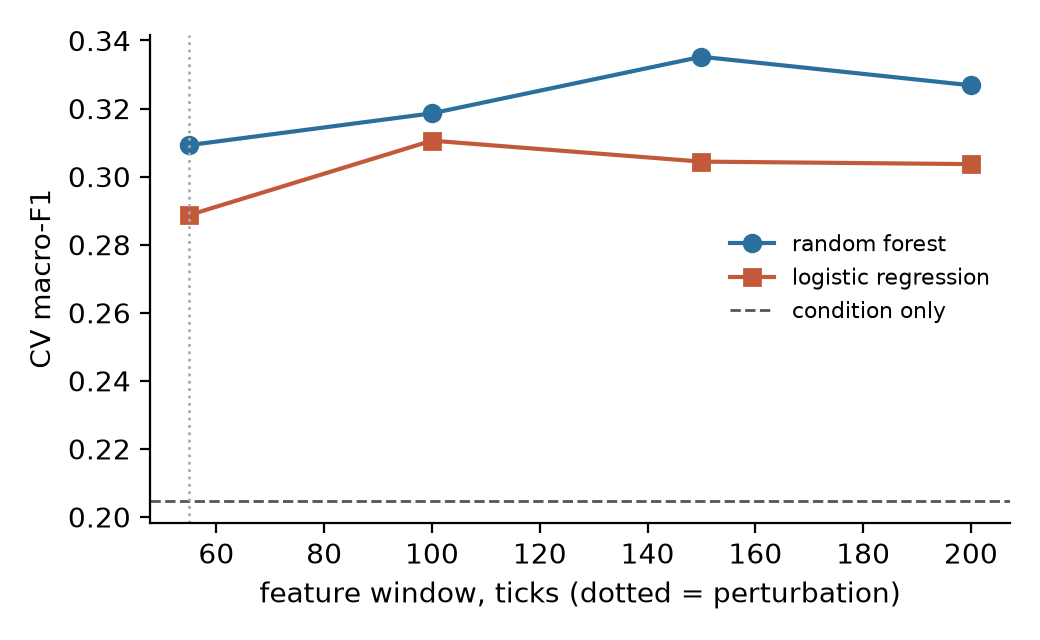
\includegraphics[width=\columnwidth]{results/horizon.png}
\caption{Cross-validated macro-F1 on the training set by length of the
feature window. The dotted line marks the perturbation at tick 55; the
dashed line is the condition-only baseline.}
\label{fig:horizon}
\end{figure}

\subsection{Threshold Sensitivity}

Across all nine combinations of stable threshold and breakdown floor the
forest scored between 0.319 and 0.362, and stayed between 0.09 and 0.19
above the condition-only model. Changing the floor from 60 to 80 per cent
moved at most 0.3 per cent of runs, because breakdown is set almost entirely
by destruction. Moving the stable threshold shifted runs between the stable
and adaptive states: the stable share was 2.8 per cent at tick 350 and 18.7
per cent at tick 550. The conclusions above hold at every setting tested.

\subsection{Feature Importance}

Permutation importance on the held-out set ranked total transmissions
first (a drop in macro-F1 of $0.020 \pm 0.012$), followed by the ratio of
most to least active agent ($0.016 \pm 0.008$) and the two AI features
($0.013 \pm 0.005$ and $0.008 \pm 0.005$). The AI features are zero in
every human-only run, so their importance is largely the AI conditions
identifying themselves. No structural or instability feature---density,
degree centralisation, rolling variance, lag-1 autocorrelation---had an
importance distinguishable from zero. Shuffling reciprocity improved the
score slightly ($-0.016 \pm 0.008$), which indicates the forest had fitted
noise in it.

\section{Discussion}

\subsection{Why Adaptation and Breakdown Did Not Separate}

The central question was whether early interaction structure indicates
whether a group will adapt or break down. In this model it largely does
not, and the reason can be traced to a single rule. Breakdown occurred when
the agent removed at tick 55 was the only holder of a required item. The
removed agent is chosen at random. A group's communication before tick 55
decides how many items are still exposed---stressed groups left more---but
not which agent is lost. Even a perfect observer of the message log could
learn only the odds of breakdown, not whether it would happen. The
information-state ceiling makes the same point from the other side: it
reached 0.641 only because it was handed the destroyed-item flag, and fell
to 0.457 without it.

This is a negative result, and the design planned for it. What it shows is
narrower than ``adaptation and breakdown cannot be told apart.'' It shows
that when disruption strikes a random member, and the group has built
little redundancy by then, breakdown is mostly luck, and a prediction
problem built on it has a low ceiling for any method. That is itself a claim
about groups, if a modest one: a team whose knowledge is concentrated can be
undone by who it happens to lose, and no amount of observation of its
communication will warn of that in advance.

\subsection{Why the Early-Warning Features Were Silent}

The instability features were chosen because critical slowing down precedes
transitions in many systems \cite{george2023}. They carried no signal here,
and that is to be expected in hindsight. Critical slowing down is a property
of a system approaching a tipping point. Integration in this model is an
accumulation: items are added and never lost except at the perturbation,
and there is no state for the group to tip out of. The model's dynamics
contain nothing for rising variance or autocorrelation to anticipate. The
qualification of Rietkerk et al.\ \cite{rietkerk2025}, that such signals do
not distinguish harmful from harmless transitions, never came into play,
because the model contains no transition of either kind for them to
precede.

\subsection{Threats to Validity}

\textit{Agent realism.} Rule-based agents have no emotion, misunderstanding,
or status concern. The study models the structure of information flow under
load, not human psychology, and results transfer to human groups only as
hypotheses requiring separate empirical test.

\textit{Self-referential validation.} Both data and labels originate in the
same simulation. The label--feature separation, the reserved calibration
seeds and the sensitivity analysis constrain but do not eliminate this
circularity \cite{larooij2025}. No claim of external validity is made.

\textit{Parameter dependence.} The proposal intended to establish findings
across a range of group sizes and item distributions. That was done only
during calibration and in the supplementary size check; the study dataset
uses one configuration. Results that depend on it, such as the exact share
of broken-down runs, should not be generalised.

\textit{A single kind of disruption.} Only the random removal of one member
was tested. Section~V-A suggests that this choice, more than any other,
determined the outcome.

\textit{A weak AI manipulation.} Because false items occupy only a
transmission and cannot crowd out or contradict genuine ones, the AI's
unreliability had little room to matter. The absence of a clear AI effect
under stress should not be read as evidence that unreliable AI is harmless
to stressed groups.

\section{Conclusion and Future Work}

This study built an agent-based model of a group pooling information under
stress, with and without an artificial participant, and asked whether the
group's early message log indicates whether it will adapt to losing a member
or break down. Stress had a clear and consistent effect on outcomes.
Classifiers on the message log beat all planned baselines, but most of what
they learned was the level of stress, and within a condition they were
close to chance. Every breakdown traced to the random loss of a member who
held something no one else had.

Four changes follow directly. \emph{Targeted perturbation}: removing the
most active or best-informed member, rather than a random one, would make
breakdown depend on structure that the features can observe, and would
test whether concentration and centralisation become predictive.
\emph{Recovery beyond completion}: labels based on time to completion
conflate slow groups with disrupted ones; comparing each run with a run from
the same seed in which no one is removed would isolate the effect of the
loss. \emph{A stronger AI manipulation}: capacity-limited agents, or false
items that contradict genuine ones, would give the AI's errors a cost, and
the trust weight could then be swept to model over- and under-reliance.
\emph{Parameter sweeps}: group size, items per agent and the timing of the
perturbation should be varied in the study data itself, not only during
calibration.

The larger aim stands: to treat collective intelligence as a trajectory and
to define failure carefully enough to predict it. What this study adds is a
worked example of how the definition of failure can decide the answer
before any model is trained.
 
\begin{thebibliography}{00}
\ifdefined\realieee\else\small\fi
\setlength{\itemsep}{6pt}
\setlength{\parsep}{0pt}
 
\bibitem{riedl2021}
C.~Riedl, Y.~J. Kim, P.~Gupta, T.~W. Malone, and A.~W. Woolley,
``Quantifying collective intelligence in human groups,'' \emph{Proc. Natl.
Acad. Sci. USA}, vol.~118, no.~21, e2005737118, 2021. Available:
\url{https://doi.org/10.1073/pnas.2005737118}
 
\bibitem{vaccaro2024}
M.~Vaccaro, A.~Almaatouq, and T.~W. Malone, ``When combinations of humans and
AI are useful: A systematic review and meta-analysis,'' \emph{Nat. Hum.
Behav.}, vol.~8, no.~12, pp.~2293--2303, 2024. Available:
\url{https://doi.org/10.1038/s41562-024-02024-1}
 
\bibitem{woolley2010}
A.~W. Woolley, C.~F. Chabris, A.~Pentland, N.~Hashmi, and T.~W. Malone,
``Evidence for a collective intelligence factor in the performance of human
groups,'' \emph{Science}, vol.~330, no.~6004, pp.~686--688, 2010. Available:
\url{https://doi.org/10.1126/science.1193147}
 
\bibitem{bates2017}
T.~C. Bates and S.~Gupta, ``Smart groups of smart people: Evidence for IQ as
the origin of collective intelligence in the performance of human groups,''
\emph{Intelligence}, vol.~60, pp.~46--56, 2017. Available:
\url{https://doi.org/10.1016/j.intell.2016.11.004}
 
\bibitem{ellis2006}
A.~P.~J. Ellis, ``System breakdown: The role of shared mental models and
transactive memory in the relationship between acute stress and team
performance,'' \emph{Acad. Manage. J.}, vol.~49, no.~3, pp.~576--589, 2006.
Available: \url{https://doi.org/10.5465/amj.2006.21794674}
 
\bibitem{staw1981}
B.~M. Staw, L.~E. Sandelands, and J.~E. Dutton, ``Threat-rigidity effects in
organizational behavior: A multilevel analysis,'' \emph{Adm. Sci. Q.},
vol.~26, no.~4, pp.~501--524, 1981. Available:
\url{https://doi.org/10.2307/2392337}
 
\bibitem{driskell1991}
J.~E. Driskell and E.~Salas, ``Group decision making under stress,''
\emph{J. Appl. Psychol.}, vol.~76, no.~3, pp.~473--478, 1991. Available:
\url{https://doi.org/10.1037/0021-9010.76.3.473}
 
\bibitem{mojzisch2025}
A.~Mojzisch, J.-H. Bahr, M.~Roswag, and J.~A. H\"ausser, ``Effects of acute
stress on group decision-making: Taking stock and looking ahead,''
\emph{Gruppe. Interaktion. Organisation.}, vol.~56, no.~3, pp.~523--536,
2025. Available: \url{https://doi.org/10.1007/s11612-025-00824-1}
 
\bibitem{vondawans2011}
B.~von Dawans, C.~Kirschbaum, and M.~Heinrichs, ``The Trier Social Stress Test
for Groups (TSST-G): A new research tool for controlled simultaneous social
stress exposure in a group format,'' \emph{Psychoneuroendocrinology},
vol.~36, no.~4, pp.~514--522, 2011.
 
\bibitem{stasser1985}
G.~Stasser and W.~Titus, ``Pooling of unshared information in group decision
making: Biased information sampling during discussion,'' \emph{J. Pers. Soc.
Psychol.}, vol.~48, no.~6, pp.~1467--1478, 1985. Available:
\url{https://doi.org/10.1037/0022-3514.48.6.1467}
 
\bibitem{stoverink2020}
A.~C. Stoverink, B.~L. Kirkman, S.~Mistry, and B.~Rosen, ``Bouncing back
together: Toward a theoretical model of work team resilience,''
\emph{Acad. Manage. Rev.}, vol.~45, no.~2, pp.~395--422, 2020. Available:
\url{https://doi.org/10.5465/amr.2017.0005}
 
\bibitem{peeters2021}
M.~M.~M. Peeters, J.~van Diggelen, K.~van den Bosch, A.~Bronkhorst,
M.~A. Neerincx, J.~M. Schraagen, and S.~Raaijmakers, ``Hybrid collective
intelligence in a human--AI society,'' \emph{AI \& Society}, vol.~36, no.~1,
pp.~217--238, 2021. Available:
\url{https://doi.org/10.1007/s00146-020-01005-y}
 
\bibitem{burton2024}
J.~W. Burton, E.~Lopez-Lopez, S.~Hechtlinger, et al., ``How large language
models can reshape collective intelligence,'' \emph{Nat. Hum. Behav.},
vol.~8, no.~9, pp.~1643--1655, 2024. Available:
\url{https://doi.org/10.1038/s41562-024-01959-9}
 
\bibitem{shiiku2025}
S.~Shiiku, R.~Marjieh, M.~Anglada-Tort, and N.~Jacoby, ``The dynamics of
collective creativity in human-AI hybrid societies,'' in \emph{Proc. 47th
Annu. Meeting Cogn. Sci. Soc.}, 2025. Available:
\url{https://arxiv.org/abs/2502.17962}
 
\bibitem{shirado2017}
H.~Shirado and N.~A. Christakis, ``Locally noisy autonomous agents improve
global human coordination in network experiments,'' \emph{Nature}, vol.~545,
no.~7654, pp.~370--374, 2017. Available:
\url{https://doi.org/10.1038/nature22332}
 
\bibitem{centola2022}
D.~Centola, ``The network science of collective intelligence,'' \emph{Trends
Cogn. Sci.}, vol.~26, no.~11, pp.~923--941, 2022. Available:
\url{https://doi.org/10.1016/j.tics.2022.08.009}
 
\bibitem{cui2024}
H.~Cui and T.~Yasseri, ``AI-enhanced collective intelligence,''
\emph{Patterns}, vol.~5, no.~11, 101074, 2024. Available:
\url{https://doi.org/10.1016/j.patter.2024.101074}
 
\bibitem{haykal2025}
D.~Haykal, M.~Goldust, H.~Cartier, and P.~Treacy, ``AI in humanitarian
healthcare: A game changer for crisis response,'' \emph{Front. Artif.
Intell.}, vol.~8, 1627773, 2025. Available:
\url{https://doi.org/10.3389/frai.2025.1627773}
 
\bibitem{gonzalo2023}
A.~Gonzalo, F.~Sanz-Garc\'ia, M.~Pelacho, A.~Taranc\'on, A.~Rivero,
O.~Varela, and A.~Moreno, ``Collective intelligence to find solutions to the
challenges posed by the Sustainable Development Goals,'' \emph{Citizen Sci.
Theory Pract.}, vol.~8, no.~1, 47, 2023. Available:
\url{https://doi.org/10.5334/cstp.587}
 
\bibitem{rossi2020}
E.~Rossi, B.~Chamberlain, F.~Frasca, D.~Eynard, F.~Monti, and M.~Bronstein,
``Temporal graph networks for deep learning on dynamic graphs,''
arXiv:2006.10637, 2020. Available: \url{https://arxiv.org/abs/2006.10637}
 
\bibitem{george2023}
S.~V. George, S.~Kachhara, and G.~Ambika, ``Early warning signals for
critical transitions in complex systems,'' \emph{Phys. Scr.}, vol.~98,
no.~7, 072002, 2023. Available:
\url{https://doi.org/10.1088/1402-4896/acde20}
 
\bibitem{rietkerk2025}
M.~Rietkerk, V.~Skiba, E.~Weinans, R.~H\'ebert, and T.~Laepple, ``Ambiguity
of early warning signals for climate tipping points,'' \emph{Nat. Clim.
Change}, vol.~15, no.~5, pp.~479--488, 2025. Available:
\url{https://doi.org/10.1038/s41558-025-02328-8}
 
\bibitem{larooij2025}
M.~Larooij and P.~T\"ornberg, ``Validation is the central challenge for
generative social simulation: A critical review of LLMs in agent-based
modeling,'' \emph{Artif. Intell. Rev.}, 2025. Available:
\url{https://doi.org/10.1007/s10462-025-11412-6}
 
 
\bibitem{suran2020}
S.~Suran, V.~Pattanaik, and D.~Draheim, ``Frameworks for collective
intelligence: A systematic literature review,'' \emph{ACM Comput. Surv.},
vol.~53, no.~1, 14, 2020. Available:
\url{https://doi.org/10.1145/3368986}
 
\bibitem{iacopini2022}
I.~Iacopini, G.~Petri, A.~Baronchelli, and A.~Barrat, ``Group interactions
modulate critical mass dynamics in social convention,'' \emph{Commun.
Phys.}, vol.~5, no.~1, 64, 2022. Available:
\url{https://doi.org/10.1038/s42005-022-00845-y}
 
\end{thebibliography}
 
\end{document}